\newpage
\section{Suggested solutions: Discrete-time Signals}
\begin{enumerate}
\item The impulse response for an LTI system is 
$$h(t)=\frac{42\sin(\omega_{c}t)}{\pi t}.$$
Let the input to the LTI system be a periodic signal with period $T=1$ of the form
$$x(t)=\sum_{n=-\infty}^{\infty}\delta(t-n).$$

\begin{enumerate}[a)]
\item Given $x(t)$ we find the Fourier transform as follows, firstly, we know that the Dirac comb can be expressed as a Fourier series of 
$$x(t)=\frac{1}{T}\sum_{n=-\infty}^{\infty}e^{i\frac{2\pi nt}{T}}.$$
In this case, we have $T=1$, hence
$$x(t)=\sum_{n=-\infty}^{\infty}e^{i2\pi nt}.$$
Thus, the Fourier series coefficients are $c_{k}=1$ for all $k\in\mathbb{Z}$. Then the Fourier transform is
$$\hat{x}(\omega)=2\pi\sum_{n=-\infty}^{\infty}\delta(\omega-2\pi n)$$
A plot of the spectrum for $\hat{x}(\omega)$ is shown in Figure \ref{diractrain} in red.

\begin{marginfigure}[1cm]
    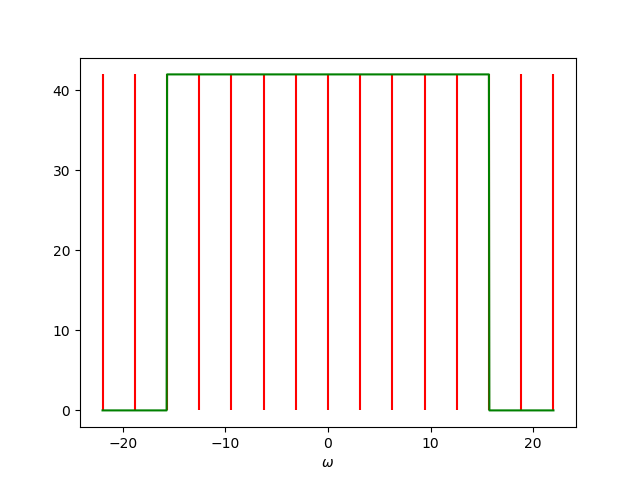
\includegraphics[height=7.5cm,width=7.0cm]{ch10/figures/diractrain.png}
    \caption{Spectrum for the Dirac comb between $-7\pi<\omega<7\pi$.}
    \label{diractrain}
\end{marginfigure}

\item The frequency response function is defined by
$$\mathcal{H}(\omega)=\mathcal{F}\{h(t)\}=\int_{-\infty}^{\infty}\frac{42\sin(\omega_{c}t)}{\pi t}e^{-i\omega t}dt=42[u(\omega+\omega_{c})-u(\omega-\omega_{c})].$$
Figure \ref{diractrain} shows the frequency response in green.


\item The output of the LTI system can be found by convolution in time domain, that is $y(t)=h(t)*x(t)$, thus, 
in frequency domain we have multiplication by the convolution theorem. By Figure \ref{diractrain} the frequencies 
inside $(-5\pi,5\pi)$ remain after multiplication, but the frequencies outside $(-5\pi,5\pi)$ gets mapped to $0$. 
In other words, the LTI system is a low pass-filter. 

\item If $y(t)=c$ then $\hat{y}(\omega)=2\pi c\delta(\omega)$ so the frequency response must then be such that
$$2\pi c\delta(\omega)=\hat{x}(\omega)\mathcal{H}(\omega)=2\pi\sum_{n=-\infty}^{\infty}\delta(\omega-2\pi n)42[u(\omega+\omega_{c})-u(\omega-\omega_{c})]=2\pi42\delta(\omega)$$
the only way for this to work is that $|\omega_{c}|\le\pi$ giving $c=42$. 
\end{enumerate}

\item Consider the running average system, defined as
$$y[n]=\mathcal{T}\{x[n]\}=\frac{1}{L}\sum_{k=0}^{L-1}x[n-k].$$

\begin{enumerate}[a)]
\item Consider two discrete-time signals $x_{1}[n]$ and $x_{2}[n]$ with arbitrary constants $c_{1},c_{2}$, then
\begin{align*}
    \mathcal{T}\{c_{1}x_{1}[n]+c_{2}x_{2}[n]\}&=\frac{1}{L}\sum_{j=0}^{L-1}[c_{1}x_{1}[n-j]+c_{2}x_{2}[n-j]] \\
    c_{1}\mathcal{T}\{x_{1}[n]\}+c_{2}\mathcal{T}\{x_{2}[n]\}&=c_{1}\frac{1}{L}\sum_{k=0}^{L-1}x_{1}[n-k]+c_{2}\frac{1}{L}\sum_{l=0}^{L-1}x_{1}[n-l]
\end{align*}
which are equal. 

For time-invariance we have
\begin{align*}
    \mathcal{T}\{\mathcal{D}\{x[n]\}\}&=\mathcal{T}\{x[n-\tau]\}=\frac{1}{L}\sum_{k=0}^{L-1}x[n-\tau-k] \\
    \mathcal{D}\{\mathcal{T}\{x[n]\}\}&=\mathcal{D}\left\{\frac{1}{L}\sum_{k=0}^{L-1}x[n-k]\right\}=\frac{1}{L}\sum_{k=0}^{L-1}x[n-\tau-k].
\end{align*}
both are equal, so the system is time-invariant. 

\item The impulse response can be determined by $h[n]=\mathcal{T}\{\delta[n]\}$, doing this yields
$$h[n]=\frac{1}{L}\sum_{k=0}^{L-1}\delta[n-k].$$
The impulse response function is then
$$h[n]=\begin{cases}
    \frac{1}{L}, \quad n=0,\hdots,L-1 \\
    0, \quad \text{otherwise}.
\end{cases}$$

\item The impulse response has $L$ nonzero values, all of them being $1/L$. 

\item Let $x[n]=e^{i\hat{\omega}_{0}n}$, then if we feed this into our system we get
$$y[n]=\frac{1}{L}\sum_{k=0}^{L-1}e^{i\hat{\omega}_{0}(n-k)}=\frac{1}{L}e^{i\hat{\omega}_{0}n}\sum_{k=0}^{L-1}e^{-i\hat{\omega}_{0}k}=\frac{1}{L}e^{i\hat{\omega}_{0}n}\left(\frac{1-(e^{-i\hat{\omega}_{0}})^{L}}{1-e^{-i\hat{\omega}_{0}}}\right).$$
The output signal is of the form $Ae^{i\phi}e^{i\hat{\omega}_{0}n}$ as $y[n]$ is then
$$y[n]=\frac{1}{L}\frac{1-e^{-i\hat{\omega}_{0}L}}{1-e^{-i\hat{\omega}_{0}}}e^{i\hat{\omega}_{0}n}=\frac{1}{L}\frac{1-e^{-i\hat{\omega}_{0}L}}{1-e^{-i\hat{\omega}_{0}}}e^{i\hat{\omega}_{0}n}$$
\end{enumerate}

\item Take $L=4$, then
$$y[n]=\frac{1}{4}\frac{1-e^{-i\hat{4\omega}_{0}}}{1-e^{-i\hat{\omega}_{0}}}x[n].$$
Next, consider the cases of input frequencies
\begin{align*}
    \hat{\omega}&=0,\\
    \hat{\omega}&=\pi,\\
    \hat{\omega}&=0.5\pi
\end{align*}
in these cases the amplitude of the output is
\begin{align*}
    A&=\lim_{\hat{\omega}\to 0}\frac{1}{4}\frac{1-e^{-4i\hat{\omega}_{0}}}{1-e^{-i\hat{\omega}_{0}}}=\lim_{\hat{\omega}\to 0}\frac{1}{4}\frac{4ie^{-4i\hat{\omega}_{0}}}{ie^{-i\hat{\omega}_{0}}}=1 \\
    A&=\frac{1}{4}\frac{1-e^{-4i\pi}}{1-e^{-i\pi}}=0,\\
    A&=\frac{1}{4}\frac{1-e^{-4i\pi/2}}{1-e^{-i\pi/2}}=0,
\end{align*}

\item The system $y[n]=\mathcal{T}\{x[n]\}$ is an LTI system and can be written as $y[n]=h[n]*x[n]$, where $h[n]$ is the impulse response function as defined above. Then the system can be described as
$$y_{2}[n]=\mathcal{T}\{\mathcal{T}\{x[n]\}\}=\mathcal{T}\{h[n]*x[n]\}=h[n]*(h[n]*x[n])=(h[n]*h[n])*x[n].$$
We've used associativity of convolution in the final step. Then the system can be described as $y_{2}[n]=h_{2}[n]*x[n]$, where $h_{2}[n]=h[n]*h[n]$, hence $y_{2}[n]$ is an LTI system as all LTI system are fully determined by convolution with an impulse response. 

\item Have that $h_{2}[n]=\mathcal{T}\{\mathcal{T}\{\delta[n]\}\}=h[n]*h[n]$, so
$$h_{2}[n]=\sum_{k=-\infty}^{\infty} h[k]h[n-k]=h[0]h[n]+h[1]h[n-1]+h[2]h[n-2]+h[3]h[n-3]+h[4]h[n-4].$$
Terms with $n<0$ are dropped as these will be $0$ due to $h[n]=0$ for $n<0$. Let's evaluate the values of $h_{2}[n]$ with $L=4$:
\begin{align*}
    h_{2}[0]&=h[0]h[0]+h[1]h[-1]+h[2]h[-2]+h[3]h[-3]+h[4]h[-4] = \frac{1}{L^{2}} \\
    h_{2}[1]&=h[0]h[1]+h[1]h[0]+h[2]h[-1]+h[3]h[-2]+h[4][-3] =\frac{2}{L^{2}} \\
    h_{2}[2]&=h[0]h[2]+h[1]h[1]+h[2]h[0]+h[3]h[-1]+h[4]h[-2] = \frac{3}{L^{2}} \\
    h_{2}[3]&=h[0]h[3]+h[1]h[2]+h[2]h[1]+h[3]h[0]+h[4]h[-1] = \frac{4}{L^{2}} \\
    h_{2}[4]&=h[0]h[4]+h[1]h[3]+h[2]h[2]+h[3]h[1]+h[4]h[0] = \frac{3}{L^{2}} \\
    h_{2}[5]&=h[0]h[5]+h[1]h[4]+h[2]h[3]+h[3]h[2]+h[4]h[1] = \frac{2}{L^{2}} \\
    h_{2}[6]&=h[0]h[6]+h[1]h[5]+h[2]h[4]+h[3]h[3]+h[4]h[2] = \frac{1}{L^{2}}
\end{align*}
while the rest are $0$. Thus
$$h_{2}[n]=\begin{cases}
    \frac{1}{16}, \quad n=0,6,\\
    \frac{2}{16}, \quad n=1,5,\\
    \frac{3}{16}, \quad n=2,4,\\
    \frac{4}{16}, \quad n=3,\\
    0, \quad \text{otherwise}.
\end{cases}$$

To draw the impulse response function, we write a little program to do it. The program is shown in Listing \ref{code12_1}. The impulse response is $0$ for all values of $n$ not shown. 
\begin{lstlisting}[language=Python, caption=Simple convolution,label=code12_1]
import numpy as n
import matplotlib.pyplot as plt

L = 4

h = n.repeat(1/L,L) # add 1/L into an array L times

h2 = n.convolve(h,h,mode="full")    # compute the convolution

plt.stem(h2)
plt.xlabel("Samples $(n)$")
plt.ylabel("$h_{2}[n]$")
plt.title("Impulse response")
plt.show()
\end{lstlisting}
The output of the program is shown in Figure \ref{h2}.

\begin{marginfigure}
    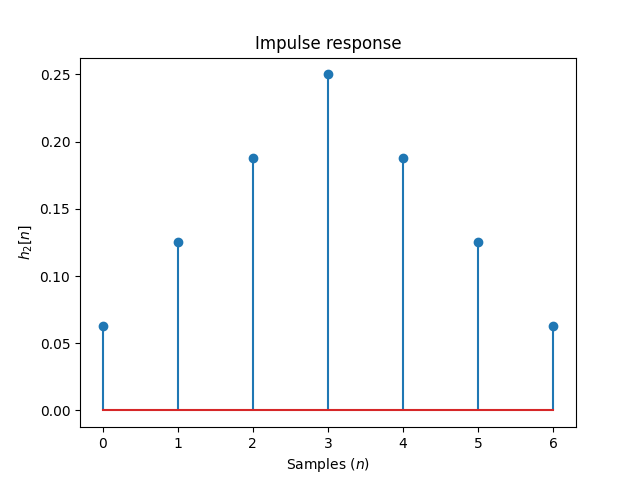
\includegraphics[width=7.5cm,height=6.5cm]{ch10/figures/h2.png}
    \caption{Impulse response for $y_{2}[n]$}
    \label{h2}
\end{marginfigure}



\end{enumerate}
